% Conference draft -- IEEE two-column. Build: cd paper && make   (needs pdflatex + bibtex + IEEEtran)
% Every number in this file comes from tables/numbers.tex or tables/tab_*.tex, which
% paper/make_assets.py generates from paper/data/. Do not type results by hand.
\documentclass[conference]{IEEEtran}
\IEEEoverridecommandlockouts
\usepackage{cite}
\usepackage{amsmath,amssymb}
\usepackage{graphicx}
\usepackage{booktabs}
\usepackage{xcolor}
\usepackage{tikz}
\usetikzlibrary{arrows.meta,positioning,fit,calc}
\usepackage[hidelinks]{hyperref}
\newcommand{\TODO}[1]{\textcolor{red}{[TODO: #1]}}
% generated by paper/make_assets.py from paper/data -- do not edit
\newcommand{\AesGcmMs}{0.01}
\newcommand{\AllDecode}{all}
\newcommand{\BenignFalse}{0/447}
\newcommand{\BenignLatency}{82}
\newcommand{\BenignPninetyfive}{278}
\newcommand{\BenignRuns}{3}
\newcommand{\CostEfive}{31.0}
\newcommand{\CostEfour}{29.5}
\newcommand{\CostEtwo}{13.4}
\newcommand{\CryptoLutShare}{54}
\newcommand{\CyclesPerPixel}{1.64}
\newcommand{\Decoders}{Pillow, OpenCV, scikit-image, FFmpeg (MJPEG)}
\newcommand{\FbDropTtm}{3.5}
\newcommand{\FpsHD}{66}
\newcommand{\FpsVGA}{199}
\newcommand{\JigsawNeighboursMax}{1.7}
\newcommand{\JigsawOracleMax}{0.47}
\newcommand{\JigsawOracleMin}{0.41}
\newcommand{\LeakEFiveMax}{0.017}
\newcommand{\LeakEFiveMin}{-0.004}
\newcommand{\LeakEOneFourMax}{0.58}
\newcommand{\LeakEOneFourMin}{0.27}
\newcommand{\LearnEfiveEdgeMax}{0.021}
\newcommand{\LearnEpochs}{25}
\newcommand{\LearnSsimMax}{0.43}
\newcommand{\LearnTest}{400}
\newcommand{\LearnTrain}{1000}
\newcommand{\MaxExtraCycles}{5}
\newcommand{\NumAttacks}{11}
\newcommand{\NumClips}{4}
\newcommand{\NumDecoders}{4}
\newcommand{\OverheadEfiveQVGA}{12}
\newcommand{\OverheadEfiveVGA}{21}
\newcommand{\OverheadEtwoQVGA}{0.5}
\newcommand{\OverheadEtwoVGA}{0.3}
\newcommand{\PolCostB}{0.162}
\newcommand{\PolCostSave}{14}
\newcommand{\PolCostT}{0.188}
\newcommand{\PolFalse}{0/6020}
\newcommand{\PolLeakB}{0.054}
\newcommand{\PolTtmB}{1.34}
\newcommand{\PolTtmT}{0.46}
\newcommand{\PyPlainMs}{134}
\newcommand{\PySelEtwoMs}{151}
\newcommand{\RealTalkFalse}{0/125}
\newcommand{\RealTalkMit}{11/11}
\newcommand{\RealTalkTtm}{1.09}
\newcommand{\RealTrailerFalse}{0/125}
\newcommand{\RealTrailerMit}{11/11}
\newcommand{\RealTrailerTtm}{0.89}
\newcommand{\ResourceSource}{a Yosys synthesis estimate}
\newcommand{\Seeds}{10}
\newcommand{\SuiteFalse}{0/375}
\newcommand{\SuiteLatency}{97}
\newcommand{\SuiteRuns}{3}
\newcommand{\TopLutPct}{10.7}
\newcommand{\TopLuts}{5{,}681}
\newcommand{\TtmMean}{0.91}
\newcommand{\TtmSd}{0.02}
\newcommand{\TurboFps}{1047}
\newcommand{\TurboMs}{0.95}


\begin{document}

\title{Playable but Private: In-Encoder Selective Encryption with Ascon-AEAD128 and Attack-Adaptive Protection for MJPEG Video on an FPGA SoC}

\author{
\IEEEauthorblockN{Aravind R, Suhas V J, Rishab H R, Samarth B N, Vijaysurya B S, Chetana G\,\TODO{order}}
\IEEEauthorblockA{Department of Electronics and Communication Engineering, RV College of Engineering, Bengaluru, India\\
\TODO{e-mails}}
}

\maketitle

\begin{abstract}
Small video cameras increasingly stream to networks they do not control, yet encrypting the whole stream makes it unplayable without the key and spends energy on every byte. We present a JPEG/MJPEG encoder for a Zynq-7020 FPGA SoC that encrypts only the sign and amplitude bits of selected DCT coefficients, at the entropy-coding stage and with a keystream from the NIST SP~800-232 lightweight standard Ascon-AEAD128. Because Huffman code lengths are untouched, every protection level remains a valid JPEG stream that common decoders open, while a 128-bit tag computed over the frame metadata and the coded scan lets the receiver reject any modified, replayed or forged frame. The register-transfer-level design is verified bit-exact against a Python golden model and needs no additional clock cycles for encryption in any mode. Around the encoder we build an authenticated feedback channel, a key ratchet and an adaptive policy that raises protection when the receiver reports attacks. In a networked simulation, all \NumAttacks{} active attacks we model were mitigated in \TtmMean{}\,s on average with no false alarms, and on \NumVideoClips{} video clips and the Kodak images a keyed block shuffle removed the outline leakage that sign and amplitude encryption alone leave behind, also against a jigsaw solver and a trained neural attacker; the same network defeats sign-only encryption. We also report a negative result: a learning bandit policy saves \PolCostSave{}\,\% of encrypted bits but reacts more slowly than a fixed threshold rule.
\end{abstract}

\begin{IEEEkeywords}
selective encryption, MJPEG, Ascon, lightweight cryptography, FPGA, authenticated encryption, video surveillance
\end{IEEEkeywords}

\section{Introduction}
Cameras on doors, corridors and machines now send video over Wi-Fi and shared Ethernet as a matter of course. Two properties matter for such a link. Confidentiality keeps a bystander on the network from watching the scene; integrity lets the viewer trust that what it shows was captured by the camera and not edited, replayed or injected on the way. The usual answer, encrypting the transport with TLS, SRTP~\cite{rfc3711} or a VPN, provides both, but it hides the stream from every tool that is not part of the key infrastructure and costs cipher work proportional to the full bitrate.

Selective encryption takes a different route: it encrypts only the parts of the compressed representation that carry most of the visual information, and leaves the format intact so that standard decoders still parse the result~\cite{massoudi2008}. For JPEG, the sign and appended amplitude bits of the DCT coefficients can be encrypted without changing any Huffman code length, so the bitstream stays compliant and its size does not grow~\cite{vandroogenbroeck2002,auer2013}. The price is that such schemes are easy to weaken: the positions of non-zero coefficients stay visible, and an attacker who guesses the hidden values can still see outlines~\cite{massoudi2008,lin2024}.

This work starts from a practical question: how much of a secure camera link can be put into the encoder hardware itself, and what does an eavesdropper still learn? We make four contributions.
\begin{enumerate}
\item An MJPEG encoder in synthesizable Verilog in which an Ascon-AEAD128~\cite{sp800232,ascon} keystream is XORed onto coefficient signs and amplitudes as they are entropy-coded, with no added cycles and closing timing at 100\,MHz on a Zynq-7020, and a per-frame tag that binds the coded scan to the protection level, session, frame counter and image size (Section~\ref{sec:design}).
\item Six protection levels, from tag-only to a keyed shuffle of macroblocks, evaluated against three keyless attackers (value replacement, a jigsaw solver and a trained U-Net) on a synthetic scene, \NumVideoClips{} real video clips (\NumOpenClips{} of them openly licensed) and the Kodak image set, together with the standard image-encryption metrics and the cost and risk of longer restart intervals (Section~\ref{sec:security}).
\item An authenticated feedback loop with a forward-secure key ratchet and an adaptive policy, evaluated against \NumAttacks{} active attacks and benign impairments; a threshold rule is compared with a contextual bandit over \Seeds{} paired seeds (Section~\ref{sec:protocol}).
\item A verification flow in which a Python golden model is the reference for every stage: Ascon matches all official known-answer tests, and every RTL block matches the model bit for bit.
\end{enumerate}

\section{Related Work}
\textit{Selective encryption of JPEG.} Van Droogenbroeck and Benedetti encrypted the appended AC bits of baseline JPEG and observed that the stream remains compliant at constant bitrate~\cite{vandroogenbroeck2002}. Puech and Rodrigues applied AES to selected DCT coefficients of medical images~\cite{puech2005}, and Auer et al.\ encrypted JPEG at bitstream level in real time with an AES-based keystream while preserving length and format~\cite{auer2013}. Massoudi et al.\ survey the field and argue that visual distortion alone is a poor proxy for security, since replacement and chosen-plaintext attacks recover much more than the scrambled image suggests~\cite{massoudi2008}. Lin et al.\ show that DCT sign bits can be recovered by optimization~\cite{lin2024}, which bounds what sign-only encryption can promise. Hirose et al.\ analyse JPEG encryption that shuffles blocks delimited by restart markers~\cite{hirose2024}; our strongest level uses the same mechanism with a keyed permutation. Selective encryption has also been extended to H.264/AVC and HEVC~\cite{boyadjis2017}.

\textit{Hardware.} Kishore et al.\ added a lightweight scrambling stage to an FPGA JPEG encoder at about 1\,\% extra hardware~\cite{kishore2015}, and Ba\u{g}baba and \"Ors combined an FPGA JPEG encoder with TEA encryption of DC and low-frequency coefficients~\cite{bagbaba2015}. Neither authenticates the frames. Ascon, now standardized by NIST in SP~800-232~\cite{sp800232,ascon}, was designed for small hardware~\cite{gross2017}; Gladis Kurian and Chen implement Ascon on an Artix-7 with Bloom-filter replay protection for IoT messages~\cite{kurian2025}.

\textit{Gap.} We found no design that (i)~places a standardized lightweight AEAD inside a hardware JPEG encoder at the entropy-coding stage, (ii)~keeps every protection level playable while authenticating each frame together with its metadata, and (iii)~closes the loop from the receiver back to the encoder so that the protection level follows observed attacks. We also could not find an evaluation of the outline leakage of such schemes against learned attackers on real video.

\section{System Design}\label{sec:design}
\begin{figure*}[t]
\centering
\resizebox{0.84\textwidth}{!}{%
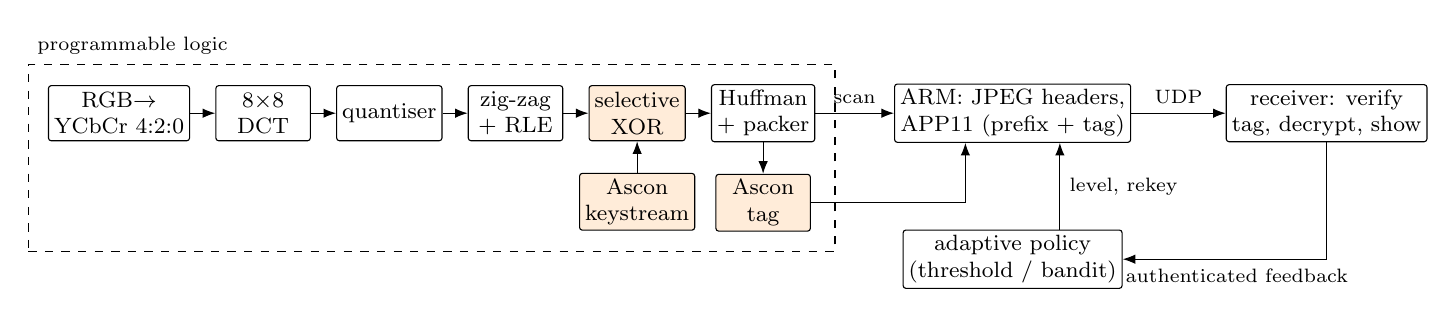
\begin{tikzpicture}[font=\footnotesize, node distance=4mm and 3.2mm,
  blk/.style={draw, rounded corners=1pt, minimum height=7mm, minimum width=12mm, align=center, inner sep=2pt},
  sec/.style={blk, fill=orange!15}, arr/.style={-{Latex[length=1.6mm]}}]
\node[blk] (cc) {RGB$\rightarrow$\\YCbCr 4:2:0};
\node[blk, right=of cc] (dct) {8$\times$8\\DCT};
\node[blk, right=of dct] (q) {quantiser};
\node[blk, right=of q] (rle) {zig-zag\\+ RLE};
\node[sec, right=of rle] (se) {selective\\XOR};
\node[blk, right=of se] (huf) {Huffman\\+ packer};
\node[sec, below=of se] (ks) {Ascon\\keystream};
\node[sec, below=of huf] (tag) {Ascon\\tag};
\draw[arr] (cc) -- (dct); \draw[arr] (dct) -- (q); \draw[arr] (q) -- (rle);
\draw[arr] (rle) -- (se); \draw[arr] (se) -- (huf); \draw[arr] (ks) -- (se);
\draw[arr] (huf) -- (tag);
\node[draw, dashed, fit=(cc)(huf)(ks)(tag), inner sep=2.5mm,
      label={[font=\scriptsize, anchor=south west]north west:programmable logic}] (pl) {};
\node[blk, right=10mm of huf] (arm) {ARM: JPEG headers,\\APP11 (prefix + tag)};
\draw[arr] (huf) -- node[above, font=\scriptsize]{scan} (arm);
\draw[arr] (tag.east) -| ([xshift=-6mm]arm.south);
\node[blk, below=11mm of arm] (pol) {adaptive policy\\(threshold / bandit)};
\draw[arr] ([xshift=6mm]pol.north) -- node[right, font=\scriptsize]{level, rekey} ([xshift=6mm]arm.south);
\node[blk, right=12mm of arm] (rx) {receiver: verify\\tag, decrypt, show};
\draw[arr] (arm) -- node[above, font=\scriptsize]{UDP} (rx);
\draw[arr] (rx.south) |- node[pos=0.72, below, font=\scriptsize]{authenticated feedback} (pol.east);
\end{tikzpicture}}
\caption{Encoder datapath with in-loop encryption (shaded) and the feedback loop. The keystream is consumed only for the fields selected by the protection level; the tag covers the frame metadata and the coded scan.}
\label{fig:system}
\end{figure*}

\subsection{Threat model}
The attacker sits on the network path. It may observe all traffic, and it may modify, drop, delay, replay or inject both video and feedback datagrams; it does not hold the keys. A passive eavesdropper sends nothing, so it cannot be detected; against it only the configured minimum protection level helps. Physical and side-channel attacks on the device are out of scope. The assets are the visual content of each frame, the integrity of content and metadata (protection level, session, counter and size), and the availability signal that tells the viewer the camera is alive. \TODO{nonce-uniqueness argument and reboot behaviour (GUIDE.md B3)}

\subsection{Encoder and cipher integration}
Fig.~\ref{fig:system} shows the datapath of a baseline JPEG encoder~\cite{t81,wallace1992}: colour conversion with 4:2:0 subsampling, a two-pass integer DCT, a reciprocal-multiplication quantiser, zig-zag ordering with run-length coding, the encryption stage, Huffman coding and a bit packer. The whole datapath is fixed-point and mirrors the golden model operation for operation, so the hardware output can be compared byte by byte.

The keystream generator runs Ascon-AEAD128 on an all-zero message under the frame nonce, one permutation round per clock cycle, and keeps a small buffer of keystream bits ahead of the encryption stage. For each coefficient the encryption stage consumes keystream bits only for the fields the protection level selects. If the sign is selected and the next keystream bit is one, all bits of the coefficient's appended amplitude field are inverted; in JPEG's one's-complement amplitude coding this is exactly a sign change. If amplitudes are selected, the remaining bits are XORed onto the lower bits of the field. The size category, and therefore the Huffman code, is never changed. As a result the encrypted scan has the same length as the plain one, and the keystream generator works in parallel with the rest of the pipeline.

A second Ascon instance computes the tag. Its associated data is a 26-byte prefix (format identifier, version, protection level, 64-bit session identifier, 64-bit frame counter, width and height) followed by every byte of the coded scan. The ARM core adds standard JPEG headers and an APP11 segment that carries the prefix and the tag; ordinary viewers skip this segment. Binding the level into the tag matters: an earlier version did not, and a frame could be downgraded undetected.

The 128-bit nonce concatenates the 64-bit session identifier with the 63-bit frame counter and one purpose bit that separates the keystream from the tag computation. The session identifier holds 48 random bits and the current key epoch.

\subsection{Protection levels}
Every level carries the per-frame tag. E0 encrypts nothing (authentication only), E1 the AC sign bits, E2 also the DC-difference signs (default minimum), E3 also the AC amplitude bits, E4 also the DC amplitude bits, and E5 adds a keyed permutation of 16$\times$16 macroblocks. Sign and amplitude encryption cannot hide which coefficients are non-zero, because the Huffman symbols reveal run lengths and size categories. E5 therefore inserts a restart marker after every macroblock and permutes the resulting segments with a Fisher--Yates shuffle driven by Ascon under a separately derived key. Restart markers keep the stream decodable but cost \OverheadEfiveQVGA--\OverheadEfiveVGA\,\% bitrate over E4 in our measurements (320$\times$240 and 640$\times$480), whereas E2 adds only the \mbox{38-byte} APP11 segment (\OverheadEtwoVGA--\OverheadEtwoQVGA\,\%). E5 is implemented in the golden model; restart-marker support in the RTL is ongoing work.

\subsection{Feedback, keys and adaptive protection}
The receiver authenticates every frame, checks the counter against a 64-entry replay window as in SRTP~\cite{rfc3711}, and returns heartbeats every 0.5\,s and rate-limited alerts. Feedback messages are themselves Ascon-AEAD128 encrypted under a separate key and protected by their own replay window. The video key is advanced by a one-way ratchet, $K_{e+1}=\mathrm{KDF}(K_e,\textrm{``ratchet''},e{+}1)$, so a key captured later does not expose earlier epochs. A dead-man rule treats three seconds without a valid heartbeat as an attack: the sender switches to the highest level and rekeys.

The sender's ARM core collects evidence in one-second windows: tag failures, replays, malformed or stale frames, frame loss over three windows, forged feedback and unexpected traffic. Two policies map this evidence to a protection level. The \emph{threshold} policy escalates to the highest level on strong evidence, holds it for 8\,s, and rekeys on bursts of tag failures. The \emph{bandit} policy is an $\varepsilon$-greedy contextual bandit~\cite{sutton2018} over a small discrete context, with optimistic initial values and sample-average updates; its reward penalizes leakage weighted by the evidence of attack, encrypted bits and level switches. Neither policy goes below the configured minimum level.

\section{Implementation and Verification}\label{sec:impl}
\begin{figure*}[t]
\centering
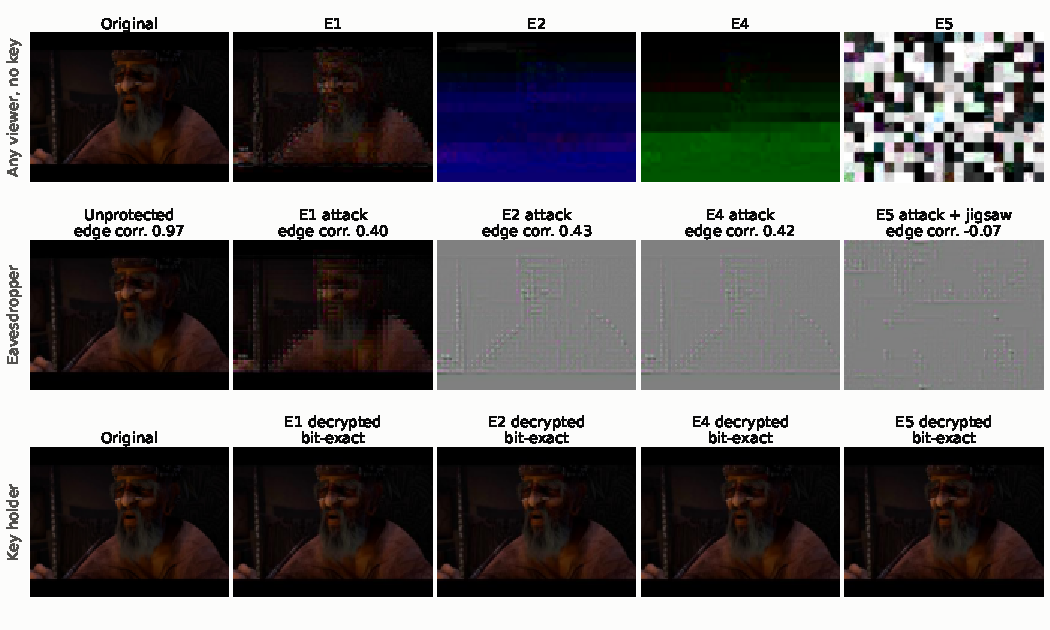
\includegraphics[width=0.62\textwidth]{figures/fig_visual_grid.pdf}
\caption{One frame of the Sintel trailer (\copyright{} Blender Foundation, CC~BY~3.0) per protection level. Top: what any viewer shows without the key. Middle: the eavesdropper's best reconstruction (replacement attack; for E5 followed by the jigsaw solver) with its edge correlation. Bottom: the key holder's output, bit-exact with the unprotected encoder.}
\label{fig:grid}
\end{figure*}
The golden model is written in Python and implements Ascon, the integer transforms, entropy coding, encryption and the container format. It passes all 1089 official Ascon-AEAD128 known-answer tests. Each RTL block has a cocotb testbench that drives random inputs with random back-pressure and compares every output with the model; the top level is compared byte for byte for E0--E4 with 64-bit session identifiers and counters above $2^{32}$. A self-checking Verilog-2001 testbench encodes five frames in all five levels and is bit-exact with the model both in Icarus Verilog and in Vivado's simulator (XSim 2026.1).

In RTL simulation of a 160$\times$128 frame, the cycle counts of E0--E4 differ by at most \MaxExtraCycles{} cycles, which is handshake noise rather than encryption work: encryption costs no cycles, and the encoder needs \CyclesPerPixel{} cycles per pixel at every level. After place and route in Vivado it meets \TopMhz\,MHz on the xc7z020 (WNS $+$\TopWns\,ns, out of context, I/O delays of 20\,\% of the period), i.e.\ \TopMpix\,Mpixel/s or \FpsVGA{} frames/s at 640$\times$480. Getting there required pipelining two paths that simulation cannot expose (a one-clock DCT row sum, first run about 47\,MHz, and a DMA-to-colour-converter path), without changing an output bit. Table~\ref{tab:resources} gives the resources (\TopLuts{} LUTs, \TopLutPct\,\% of the device; about \TopPowerMw\,mW, vectorless estimate). The two Ascon instances take \CryptoLutShare\,\% of the LUTs, and all \ConvBram{} BRAM36 are the converter's MCU-row buffers, sized for 2048-pixel lines. In Table~\ref{tab:compare}, each of our Ascon cores (\AsconLutMin--\AsconLutMax{} LUTs) is as small as the round-per-cycle Ascon-p cores of~\cite{khairallah2023}, and our JPEG datapath uses fewer LUTs than the commercial encoders~\cite{logijpge,castjpeg}, which however process one sample per clock at 150--166\,MHz with less block RAM.

% generated by paper/make_assets.py from paper/data -- do not edit
\begin{table}[t]
\caption{Resources on the xc7z020 (53\,200 LUT, 106\,400 FF, 140 BRAM36, 220 DSP). Source: Vivado post-route, out of context, 100\,MHz with I/O delays of 20\,\% of the period, WNS +0.630\,ns.}
\label{tab:resources}
\centering\small
\resizebox{\columnwidth}{!}{%
\begin{tabular}{lrrrr}
\toprule
Block & LUT & FF & BRAM36 & DSP \\
\midrule
Encoder (all) & 4785 (9.0\%) & 3051 (2.9\%) & 25.5 (18.2\%) & 23 (10.4\%) \\
\quad colour conversion + line buffers & 459 & 220 & 25 & 0 \\
\quad DCT and quantizer & 806 & 69 & 0 & 22 \\
\quad zig-zag, Huffman, packing & 717 & 323 & 0 & 0 \\
\quad keystream generator (Ascon) & 949 & 851 & 0 & 0 \\
\quad tag unit (Ascon) & 1358 & 1072 & 0 & 0 \\
\quad selective encryption & 82 & 24 & 0 & 0 \\
\quad AXI-Lite registers & 392 & 451 & 0 & 0 \\
\bottomrule
\end{tabular}}
\end{table}

% generated by paper/make_assets.py from paper/data -- do not edit
\begin{table}[t]
\caption{Comparison with published FPGA designs. Their numbers are as reported by each source; ours are
post-route (Table~\ref{tab:resources}) with throughput from the RTL cycle count. Mpx/s: million pixels per second.}
\label{tab:compare}
\centering\small
\resizebox{\columnwidth}{!}{%
\begin{tabular}{llrrrrrl}
\toprule
Design & Device & LUT & BRAM & DSP & MHz & Mpx/s & Crypto \\
\midrule
Ours: encoder & Zynq-7020 & 5{,}039 & 24.5 & 23 & 100 & 61 & sel.\ AEAD \\
Ours: one Ascon & Zynq-7020 & 860--969 & 0 & 0 & 100 & -- & AEAD core \\
logiJPGE~\cite{logijpge} & Zynq-7020 & 3{,}240 & 16 & 30 & 150 & 150 & none \\
CAST JPEG-E-S~\cite{castjpeg} & Artix-7 & 3{,}069 & 2 & 16 & 166 & -- & none \\
Khairallah~\cite{khairallah2023} & Artix-7 & 1{,}031 & 0 & 0 & 200 & -- & MAC \\
Kurian~\cite{kurian2025} & Artix-7 & 5{,}335 & 32 & 0 & 100 & -- & AEAD \\
\bottomrule
\end{tabular}}
\end{table}


\section{Security Evaluation}\label{sec:security}
\textit{Setup.} We measure what a keyless observer can reconstruct. For every frame we take the better of two pictures: the protected stream decoded as is, and a \emph{replacement attack} that substitutes fixed guesses for the encrypted values (absolute values for encrypted signs, the smallest value of the size category for encrypted amplitudes, zero DC differences) and re-encodes a valid JPEG. Leakage is the Pearson correlation between the Sobel gradient magnitudes of this picture and of the original (edge correlation); we also report SSIM~\cite{ssim}. Sources are a synthetic corridor scene; \NumClips{} publicly available HD clips that we analyse but do not reproduce (two film trailers and two talking-head videos, identified by hash); \NumOpenClips{} openly licensed films of the Blender Foundation, the Sintel trailer and Tears of Steel (CC~BY~3.0)\footnote{\url{https://durian.blender.org}, \url{https://mango.blender.org}}; and the 24 images of the Kodak set\footnote{\url{http://r0k.us/graphics/kodak/}}. Video is resized to 320$\times$240 and sampled every 150 frames; frames without edges are excluded.

\textit{Format compliance.} The protected streams of \AllDecode{} six levels decode without error in \Decoders{}, at the original resolution.


\textit{Outline leakage.} Fig.~\ref{fig:grid} and Table~\ref{tab:leakage} show the main effect. Under E1--E4 the eavesdropper sees a clear outline of the scene: edge correlation stays between \LeakEOneFourMin{} and \LeakEOneFourMax{} on the real sources, and encrypting amplitudes in addition to signs (E3, E4) does not reduce it, because the positions and size categories of the non-zero coefficients remain public. The keyed macroblock permutation of E5 removes the outline (edge correlation between \LeakEFiveMin{} and \LeakEFiveMax{}). In terms of cost, E2 encrypts \CostEtwo\,\% of the bits, E4 \CostEfour\,\%, and E5 only slightly more, \CostEfive\,\%, yet only E5 moves leakage to zero.

% generated by paper/make_assets.py from paper/data -- do not edit
\begin{table}[t]
\caption{Outline leakage: edge correlation between the original and the eavesdropper's best keyless reconstruction (decode or replacement attack; 0 = no outline), up to 20 frames per source; frames without edges are skipped. The first row is the fraction of payload bits encrypted.}
\label{tab:leakage}
\centering\small\setlength{\tabcolsep}{4pt}
\resizebox{\columnwidth}{!}{%
\begin{tabular}{lrrrrrr}
\toprule
Source & E0 & E1 & E2 & E3 & E4 & E5 \\
\midrule
Enc.\ share & 0.00 & 0.11 & 0.13 & 0.26 & 0.30 & 0.31 \\
\midrule
Synthetic & 1.00 & 0.38 & 0.36 & 0.37 & 0.37 & 0.00 \\
Trailer A & 0.99 & 0.47 & 0.34 & 0.34 & 0.33 & 0.01 \\
Trailer B & 0.99 & 0.58 & 0.27 & 0.31 & 0.30 & 0.02 \\
Talk A & 0.99 & 0.50 & 0.44 & 0.44 & 0.44 & -0.00 \\
Talk B & 0.99 & 0.49 & 0.38 & 0.44 & 0.43 & 0.01 \\
Sintel & 0.99 & 0.35 & 0.25 & 0.26 & 0.27 & -0.00 \\
Tears of Steel & 0.99 & 0.47 & 0.34 & 0.35 & 0.43 & -0.01 \\
Kodak & 0.99 & 0.39 & 0.32 & 0.33 & 0.30 & 0.00 \\
\bottomrule
\end{tabular}}
\end{table}


\textit{Jigsaw attacker.} A permutation of blocks invites a puzzle solver. Our greedy region-growing solver in the style of~\cite{pomeranz2011} restores most neighbour relations on unencrypted shuffled tiles. On E5 replacement-attack tiles it places at most \JigsawNeighboursMax\,\% of neighbour pairs correctly, and the solved picture has no outline (Table~\ref{tab:leakage}). The structure is not destroyed, only hidden: an oracle that knew the permutation would recover edge correlations of \JigsawOracleMin--\JigsawOracleMax. A stronger solver may do better, so this bounds the leakage from below only.

\textit{Learned attacker.} We trained a U-Net~\cite{unet} to map the two keyless pictures (decoded and replacement attack) to the original and always tested it on clips it had not seen (Table~\ref{tab:learned}). P1 and P2 train on \LearnTrain{} frames of one clip, P3 uses only the open films, and P4 trains a wider network for \LearnBigEpochs{} epochs on \LearnBigTrain{} frames of three clips and tests on \LearnBigTest{} frames of three others. The network defeats sign-only encryption: under E1 it reaches an edge correlation of \LearnEoneEdge{} and SSIM \LearnEoneSsim{} (replacement attack: \ReplEoneEdge{}), so E1 is no protection against a trained attacker. Under E2 and E4 it adds little to the outline that replacement already reveals (edge correlation \LearnEtwoFourEdgeMin--\LearnEtwoFourEdge{} against \ReplEtwoFourEdge) but raises SSIM to about \LearnEtwoFourSsimBig{} by learning brightness and colour. As a control we score the median training frame, which uses no ciphertext (last row of Table~\ref{tab:learned}). Under E5 the network's edge correlation (\LearnEfiveEdgeBig, 95\,\% interval \LearnEfiveCiLo--\LearnEfiveCiHi) equals that of this prior (\CtrlEdgeBig), so no outline comes from the stream; its SSIM exceeds the prior by \LearnEfiveGain{} in P4, while in P3 it matches it (\OpenEfiveSsim{} vs.\ \OpenCtrlSsim); we attribute the gain to frame-level brightness and colour statistics, which a permutation of blocks does not hide. We therefore claim that E5 hides the shape of the scene from these attackers, not that it hides everything.

\textit{Restart interval.} E5 as specified costs \RiOverheadOneMin--\RiOverheadOneMax\,\% over the same E4 coefficients at 320$\times$240, because every macroblock ends with a two-byte marker and restarts DC prediction. $N$ macroblocks per segment reduce this to \RiOverheadFour\,\% at $N{=}4$ and \RiOverheadThirtyTwo\,\% at $N{=}32$ (Table~\ref{tab:restart}). Hirose et al.\ showed that a non-zero counting attack (NZCA) reveals the scene from the run-length symbols, which no level encrypts~\cite{hirose2024}. Without the shuffle, our NZCA map correlates \RiNzcaEfourMin--\RiNzcaEfourMax{} with the original's block edge energy; with it, at most \RiNzcaEfiveMax{} for every $N$ we tried. Global correlations understate large segments, however: at $N{=}32$ only \RiSegThirtyTwo{} segments remain, each an intact strip of 32 macroblocks, and a beam-search solver that chains segments by border continuity links \RiSuccThirtyTwoMin--\RiSuccThirtyTwoMax{} of them to their true successor on the real clips (chance \RiChanceThirtyTwo), against at most \RiSuccSmallMax{} for $N\le 8$. We keep $N{=}1$ and do not claim that longer intervals are safe.

\textit{Standard metrics.} We also computed the usual image-encryption metrics on all \StdSources{} sources (5--6 frames each; full table in our repository). Key sensitivity holds: decrypting E5 with a key that differs in one bit changes \StdNpcrEfiveMin--\StdNpcrEfiveMax\,\% of the pixels, with SSIM at most \StdWrongSsimEfiveMax. The other metrics assume a cipher that turns the image into noise, which a format-compliant scheme does not: the 8$\times$8 block structure survives, so adjacent-pixel correlation stays at \StdCorrMin--\StdCorrMax{} (0 for a full cipher) and entropy rises only under E5 (\StdEntropyPlain{} to \StdEntropyEfive{} bits). The 1-pixel NPCR (at most \StdPixelNpcrMax\,\%) measures diffusion, which a stream cipher lacks by design and which a fresh nonce per frame makes irrelevant. We report these values for comparability, not as evidence of security.

% generated by paper/make_assets.py from paper/data -- do not edit
\begin{table}[t]
\caption{U-Net reconstruction, SSIM / edge corr.\ on unseen test clips. P1: Trailer A$\rightarrow$B, P2: Talk A$\rightarrow$B, P3: Sintel$\rightarrow$Tears of Steel, P4: three clips$\rightarrow$three others. Repl.: replacement attack, P4 test set.}
\label{tab:learned}
\centering\small\setlength{\tabcolsep}{3pt}
\resizebox{\columnwidth}{!}{%
\begin{tabular}{llcccc}
\toprule
Mode & Repl. & P1 & P2 & P3 & P4 \\
\midrule
E1 & 0.55 / 0.40 & 0.72 / 0.53 & 0.70 / 0.66 & 0.55 / 0.42 & 0.79 / 0.69 \\
E2 & 0.17 / 0.40 & 0.42 / 0.33 & 0.27 / 0.34 & 0.13 / 0.32 & 0.34 / 0.40 \\
E4 & 0.18 / 0.39 & 0.43 / 0.34 & 0.28 / 0.32 & 0.12 / 0.26 & 0.35 / 0.40 \\
E5 & 0.14 / 0.00 & 0.34 / -0.02 & 0.26 / 0.02 & 0.22 / 0.00 & 0.36 / 0.04 \\
\bottomrule
\end{tabular}}
\end{table}

% generated by paper/make_assets.py from paper/data -- do not edit
\begin{table}[t]
\caption{E5 with $N$ macroblocks per restart segment, mean over 5 sources at 320$\times$240. Overhead: bytes over the same E4 coefficients without markers. NZCA: correlation of the per-block count of non-zero coefficients with the original's block edge energy. Succ.: share of segments a beam-search solver chains to their true successor (chance in brackets).}
\label{tab:restart}
\centering\small\setlength{\tabcolsep}{3.5pt}
\resizebox{\columnwidth}{!}{%
\begin{tabular}{lccccc}
\toprule
$N$ & Segments & Perm.\ bits & Overhead (\%) & NZCA & Succ.\ (chance) \\
\midrule
E4 (no shuffle) & -- & -- & -- & 0.82 & -- \\
1 & 300 & 2041 & 15.2 & 0.01 & 0.02 (0.00) \\
2 & 150 & 873 & 7.5 & 0.01 & 0.03 (0.01) \\
4 & 75 & 363 & 3.8 & 0.02 & 0.04 (0.01) \\
8 & 38 & 149 & 1.9 & 0.02 & 0.03 (0.03) \\
10 & 30 & 108 & 1.5 & 0.02 & 0.08 (0.03) \\
32 & 10 & 22 & 0.5 & 0.04 & 0.27 (0.11) \\
\bottomrule
\end{tabular}}
\end{table}


\section{Protocol and Defence Evaluation}\label{sec:protocol}
\textit{Setup.} Sender, network channel, receiver and logger run as separate processes that talk over UDP, so the evaluation exercises the real wire format, fragmentation and timing. The sender encodes 320$\times$240 video at 10 frames/s with the golden model (same bytes as the RTL). The channel can impose loss, delay, jitter and reordering, and it implements the attacker of our threat model. All results below come from a 4-core cloud virtual machine with one scenario running at a time.

\textit{Active attacks.} The full scenario applies \NumAttacks{} attacks for six seconds each, 25\,s apart: bit flips in the scan, a mode downgrade in the header, splicing of two frames, injection of a forged frame, replay, delay, dropping, a junk flood, and dropping, forging and replaying feedback. Table~\ref{tab:attacks} gives the result over \SuiteRuns{} runs. Every attack was mitigated in every run, on average \TtmMean{}\,$\pm$\,\TtmSd{}\,s after it began, with \SuiteFalse{} false alarms in calm windows and a median frame latency of \SuiteLatency\,ms. The slowest case, dropped feedback, is caught only by the dead-man rule, after about \FbDropTtm\,s: the 3\,s timeout plus part of a decision window. With a trailer, a talking-head clip or Tears of Steel as the video source instead of the synthetic scene, all attacks were again mitigated (\RealTrailerMit{}, \RealTalkMit{} and \RealOpenMit{}; means \RealTrailerTtm{}, \RealTalkTtm{} and \RealOpenTtm{}\,s, one run each) without false alarms.

\textit{Benign impairments.} A second scenario applies only network problems: rising packet loss up to 6\,\%, delay up to 120\,ms with jitter, and 5\,\% reordering. Over \BenignRuns{} runs the defence raised no false alarm (\BenignFalse{} windows); median latency was \BenignLatency\,ms and the 95th percentile \BenignPninetyfive\,ms. Two design choices made this possible: loss is judged over three windows instead of one, and late frames are distinguished from replays by the replay window.

% generated by paper/make_assets.py from paper/data -- do not edit
\begin{table}[t]
\caption{Reaction to each active attack (full suite, threshold policy, 3 runs; mean\,$\pm$\,s.d. in seconds). ``First rejection'' is when the receiver first discards a frame; ``mitigated'' is when the sender has raised protection or rekeyed.}
\label{tab:attacks}
\centering\small\setlength{\tabcolsep}{4pt}
\resizebox{\columnwidth}{!}{%
\begin{tabular}{lccc}
\toprule
Attack & Mitigated & First rejection & Mitigated after \\
\midrule
bit flips in the scan & 3/3 & 0.09\,$\pm$\,0.03 & 0.41\,$\pm$\,0.02 \\
mode downgrade in header & 3/3 & 0.06\,$\pm$\,0.02 & 0.44\,$\pm$\,0.02 \\
splice of two frames & 3/3 & 0.13\,$\pm$\,0.00 & 0.46\,$\pm$\,0.01 \\
forged frame injection & 3/3 & 0.14\,$\pm$\,0.06 & 0.44\,$\pm$\,0.03 \\
frame replay & 3/3 & 0.07\,$\pm$\,0.05 & 0.46\,$\pm$\,0.03 \\
frame delay & 3/3 & 4.13\,$\pm$\,0.04 & 1.46\,$\pm$\,0.03 \\
frame dropping & 3/3 & -- & 1.46\,$\pm$\,0.03 \\
junk flood & 3/3 & -- & 0.49\,$\pm$\,0.04 \\
feedback dropping & 3/3 & -- & 3.47\,$\pm$\,0.05 \\
forged feedback & 3/3 & -- & 0.46\,$\pm$\,0.04 \\
feedback replay & 3/3 & -- & 0.44\,$\pm$\,0.01 \\
\bottomrule
\end{tabular}}
\end{table}


\textit{Threshold rule against bandit.} The learning scenario repeats a bit-flip and a replay attack five times each, separated by calm periods. We ran both policies with \Seeds{} paired seeds. Table~\ref{tab:policies} shows a consistent trade-off rather than a winner. The bandit encrypted fewer bits in every seed (\PolCostB{} against \PolCostT{} of the payload, \PolCostSave\,\% less), but it reacted later (\PolTtmB{} against \PolTtmT\,s) and leaked more while attacks were active (\PolLeakB{} against almost zero), again in every seed. Neither policy raised a false alarm (\PolFalse{}). For a security link we keep the threshold rule as the default and treat the bandit as an option where bandwidth or energy matters more than the first second of an attack.

% generated by paper/make_assets.py from paper/data -- do not edit
\begin{table}[t]
\caption{Threshold rule vs.\ $\varepsilon$-greedy bandit on the learning scenario, 10 seeds each (mean\,$\pm$\,s.d.). The last column counts the seeds in which the bandit was better (lower) than the threshold rule with the same seed.}
\label{tab:policies}
\centering\small\setlength{\tabcolsep}{4pt}
\resizebox{\columnwidth}{!}{%
\begin{tabular}{lccc}
\toprule
Metric & Threshold & Bandit & Bandit better \\
\midrule
Mitigation (s) & 0.46\,$\pm$\,0.02 & 1.34\,$\pm$\,0.03 & 0/10 \\
Leakage under attack & 0.000\,$\pm$\,0.001 & 0.054\,$\pm$\,0.004 & 0/10 \\
Encrypted share & 0.188\,$\pm$\,0.001 & 0.162\,$\pm$\,0.001 & 10/10 \\
Encrypted share, calm & 0.135\,$\pm$\,0.000 & 0.138\,$\pm$\,0.001 & 0/10 \\
\bottomrule
\end{tabular}}
\end{table}


\textit{Cost relative to software.} On the simulation host, our Python model needs \PyPlainMs\,ms to encode a 640$\times$480 frame and \PySelEtwoMs\,ms including E2 selective encryption, whereas libjpeg-turbo takes \TurboMs\,ms and full-stream AES-GCM about \AesGcmMs\,ms. A desktop processor is therefore not the right comparison; the case for the encoder rests on the SoC's embedded processor, which has no AES instructions, and on output that stays playable and authenticated. \TODO{ARM Cortex-A9 baseline (libjpeg-turbo, AES-GCM, selective encryption in C), FPGA frame rate and energy per frame measured on the PYNQ-Z2 (GUIDE.md A1--A4, B1)}

\section{Discussion and Limitations}
Three limitations bound our claims. First, our hardware numbers are post-route for the encoder alone and the power figure is a vectorless estimate; timing closure of the complete Zynq system and measurements on the board are pending, and E5 exists only in the golden model. Second, sign and amplitude encryption leak outlines by construction, however many bits are encrypted; only a change of block positions removes them, at a bitrate cost. Third, our attackers are greedy or trained on a few clips; stronger puzzle solvers or attackers trained on large video corpora may extract more from E5, and a trained network already undoes sign-only encryption (E1). On the protocol side, the receiver cannot tell heavy benign loss from partial jamming, so only near-total suppression escalates, and the reaction time is bounded below by the one-second decision window.

\section{Conclusion}
Encrypting coefficient signs and amplitudes with Ascon inside a JPEG encoder costs no cycles, keeps every protection level playable, and, combined with a per-frame tag over metadata and scan, turns a plain MJPEG stream into an authenticated one. Our measurements also show the limit of the idea: without a keyed change of block positions, an eavesdropper still sees the outline of the scene, whatever share of bits is encrypted. A closed feedback loop detects and answers active attacks within about a second in simulation. The next steps are on-board results on the PYNQ-Z2, macroblock shuffling in hardware, a shared Ascon core, key derivation with the standard's extendable-output function instead of the AEAD tag, and learned attackers trained on large video corpora.

\section*{Acknowledgment}
We thank Dr.~Chetana~G for her guidance. \TODO{AI-assistance disclosure as required by the conference (see paper/README.md): name the tools and what they were used for, e.g. code generation, test scaffolding and language editing.}

\bibliographystyle{IEEEtran}
\bibliography{refs}

\end{document}
